\section{环和理想}

参见 Atiyah, \href{https://phanpu.github.io/2021/12/26/a-rough-reading-note-for-atiyah-s-commutative-algebra/Commutative_Algebra_Atiyah.pdf}{Commutative\_Algebra\_Atiyah.pdf}

\begin{exercise}
设 $A$ 是环, 令
\[
f = a_{0} + a_{1} x + \cdots + a_{n} x^{n} \in A[x]
\]证明:
	\begin{enumerate}
		\item $f$ 是 $A[x]$ 的可逆元 $\Leftrightarrow a_{0}$ 是 $A$ 中可逆元且 $a_{1}, \cdots, a_{n}$ 是幂零元。
		\item $f$ 幂零 $\Leftrightarrow a_{0}, a_{1}, \cdots, a_{n}$ 幂零。
		\item $f$ 是零因子 $\Leftrightarrow$ 存在着环 $A$ 的非 0 元 $a$ 使得 $a f = 0$。
		\item 如果 $(a_{0}, \cdots, a_{n}) = (1)$, $f$ 就叫本原多项式。证明: 如果 $f, g \in A[x]$, 那么 $f g$ 本原 $\Leftrightarrow f, g$ 均为本原。
	\end{enumerate}
\end{exercise}
\begin{proof}

\begin{enumerate}
	\item $\Leftarrow$: 设 $a_{i}^{m_{i}} = 0, 1 \leq i \leq n$, 不妨 $a_{0} = 1$, 否则考虑 $a_{0}^{-1} f$, 则 $(f-1)^{m_{1}+\cdots+m_{n}} = 0$, 记幂数为 $M$, 从而 $1 = 1-(1-f)^{M} = f((1-f)^{M-1}+\cdots+1)$。(实际上就是题 1)
\end{enumerate}

$\Rightarrow$: 设 $f g = 1$, 且 $g(x) = b_{0}+b_{1} x+\cdots+b_{m} x^{m}$, 令 $x=0$, 可得 $a_{0} b_{0} = 1$, 从而 $a_{0}$ 可逆。

从而有 $\forall k, \sum_{i+j=k} a_{i} b_{j} = 0$(线性代数的结论), 特别的 $a_{n} b_{m} = 0$, $a_{n} b_{m-1} + b_{m} a_{n-1} = 0$, 从而 $a_{n}^{2} b_{m-1} = 0$, 如此往下, $a_{n}^{m+1} b_{0} = 0$, 故 $a_{n}$ 幂零。对其余同理。(由于 $a_n$ 幂零,则 $a_nx^{n}$ 幂零,故 $f-a_nx^{n}=\sum_{i=0}^{n-1}a_ix^{i}\eqqcolon f_1$ 依然可逆,对 $f_1$ 重复上述论证可得 $a_{n-1}$ 幂零,依此类推)
\end{proof}

\section{模与理想}

\begin{proposition}
极大理想都是素理想.
\end{proposition}
\begin{exercise}
$(N:P)=\text{Ann}((P+N)/N)$.
\end{exercise}
\begin{note}
这里使用 $\text{Ann}((P+N)/N)$ 而不是 $\text{Ann}(P/N)$,是因为后者只在 $N\subset P$ 的情况下有定义,而前者总是良好定义的.
\end{note}
\begin{exercise}
\begin{figure}[H]
\centering
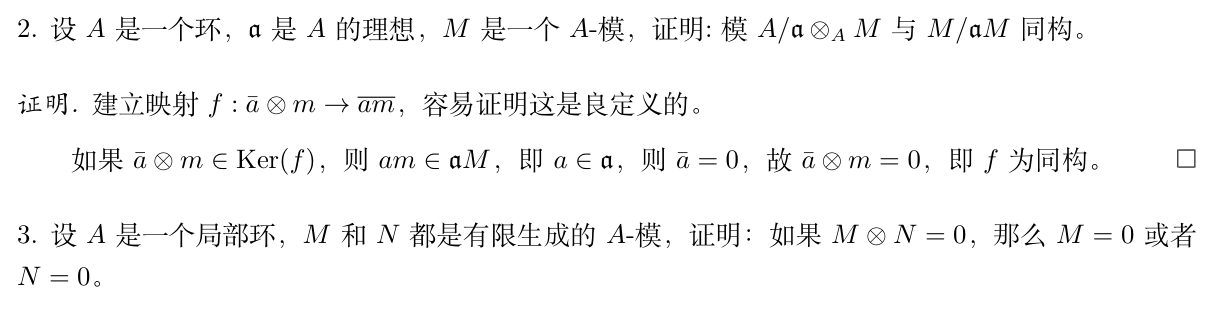
\includegraphics[width=\textwidth]{交换代数-2025052111.png}
% \caption{}
\label{}
\end{figure}
\begin{figure}[H]
\centering
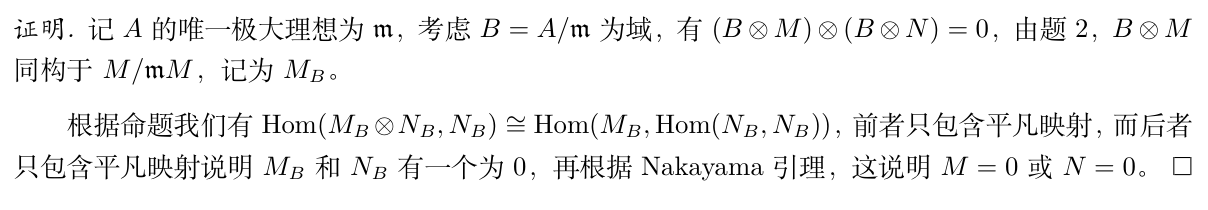
\includegraphics[width=\textwidth]{1-交换代数-2025052111.png}
% \caption{}
\label{}
\end{figure}
\end{exercise}
解释 3 的证明:

这个证明的目的是要说明:在一个局部环 $A$ 上,如果两个有限生成的 $A$-模 $M$ 和 $N$ 的张量积 $M \otimes_A N = 0$,那么 $M$ 和 $N$ 中至少有一个是零模。

证明过程可以分解为以下几个步骤:

\subsection{证明步骤详解}

\textbf{引入剩余域 (Residue Field)}

设 $A$ 是一个局部环,其唯一的极大理想为 $\mathfrak{m}$。

考虑 $B = A/\mathfrak{m}$。因为 $\mathfrak{m}$ 是极大理想,所以 $B$ 是一个域,称为 $A$ 的\textbf{剩余域}。

\textbf{张量积与剩余域}

我们已知 $M \otimes_A N = 0$。

将这个等式两边都用 $B = A/\mathfrak{m}$ 在 $A$ 上作张量积,可以得到:
\[
(A/\mathfrak{m}) \otimes_A (M \otimes_A N) = (A/\mathfrak{m}) \otimes_A 0 = 0
\]
利用张量积的结合律和换环定理 (change of rings, $R \otimes_A (M \otimes_A N) \cong (R \otimes_A M) \otimes_R (R \otimes_A N)$,其中 $R$ 是一个 $A$-代数),这里 $R=B=A/\mathfrak{m}$,我们有:
\[
( (A/\mathfrak{m}) \otimes_A M ) \otimes_{A/\mathfrak{m}} ( (A/\mathfrak{m}) \otimes_A N ) = 0
\]
根据题目2的结论 ($A/\mathfrak{a} \otimes_A M \cong M/\mathfrak{a}M$),我们知道:

\begin{itemize}
	\item $B \otimes_A M \cong M/\mathfrak{m}M$。我们记 $M_B = M/\mathfrak{m}M$。
	\item $B \otimes_A N \cong N/\mathfrak{m}N$。我们记 $N_B = N/\mathfrak{m}N$。
\end{itemize}

因此,上面的等式变为 $M_B \otimes_B N_B = 0$。 注意 $M_B$ 和 $N_B$ 都是域 $B$ 上的向量空间。

\textbf{向量空间的张量积}

我们得到了 $M_B \otimes_B N_B = 0$,其中 $M_B$ 和 $N_B$ 是域 $B$ 上的向量空间。

对于域上的向量空间 $V, W$,如果 $V \otimes_B W = 0$,那么必然有 $V=0$ 或者 $W=0$。(如果 $V, W$ 均非零,它们分别有非空基底,则 $V \otimes_B W$ 的基底由它们基底元素的张量积构成,因此 $V \otimes_B W$ 也非零。)

证明中使用了Hom函子的性质来推导这一结论:

\begin{itemize}
	\item 利用张量-Hom伴随 (tensor-hom adjunction):
\[
\text{Hom}_B(M_B \otimes_B N_B, N_B) \cong \text{Hom}_B(M_B, \text{Hom}_B(N_B, N_B))
\]	\item 由于 $M_B \otimes_B N_B = 0$,那么左边的 $\text{Hom}_B(0, N_B)$ 只包含零映射(从零空间到 $N_B$ 的唯一线性映射是零映射)。
	\item 因此,右边的 $\text{Hom}_B(M_B, \text{Hom}_B(N_B, N_B))$ 也必须为零(即只包含零映射)。
	\item 对于域 $B$ 上的向量空间 $X$ 和 $Y$,如果 $\text{Hom}_B(X, Y) = 0$,那么 $X=0$ 或者 $Y=0$。(如果 $X \ne 0$ 且 $Y \ne 0$,我们可以构造一个非零的从 $X$ 到 $Y$ 的线性映射)。
	\item 所以,从 $\text{Hom}_B(M_B, \text{Hom}_B(N_B, N_B)) = 0$ 可以得出:
$M_B = 0$ 或者 $\text{Hom}_B(N_B, N_B) = 0$。
	\item 如果 $\text{Hom}_B(N_B, N_B) = 0$,这意味着从 $N_B$ 到 $N_B$ 的唯一线性映射是零映射。但如果 $N_B \ne 0$,那么其上的恒等映射 $id_{N_B}$ 就不是零映射。所以,$\text{Hom}_B(N_B, N_B) = 0$ 必然意味着 $N_B = 0$。
	\item 综上,我们得出结论:$M_B = 0$ 或者 $N_B = 0$。也就是 $M/\mathfrak{m}M = 0$ 或者 $N/\mathfrak{m}N = 0$。
\end{itemize}

\textbf{应用中山正引理 (Nakayama's Lemma)}

我们已知 $A$ 是一个局部环,$\mathfrak{m}$ 是其唯一的极大理想。$M$ 和 $N$ 是有限生成的 $A$-模。

中山正引理的一个形式是:若 $M$ 是环 $A$ 上的有限生成模,$I$ 是 $A$ 的一个理想且 $I$ 包含于 $A$ 的 Jacobson 根 $J(A)$ 中。如果 $IM=M$,则 $M=0$。

对于局部环 $A$,其 Jacobson 根就是其唯一的极大理想 $\mathfrak{m}$。

所以:

\begin{itemize}
	\item 如果 $M/\mathfrak{m}M = 0$,这意味着 $M = \mathfrak{m}M$。由于 $M$ 是有限生成的 $A$-模,根据中山正引理,可得 $M=0$。
	\item 同理,如果 $N/\mathfrak{m}N = 0$,这意味着 $N = \mathfrak{m}N$。由于 $N$ 是有限生成的 $A$-模,根据中山正引理,可得 $N=0$。
\end{itemize}

\textbf{结论}

因为我们已经证明了 $M/\mathfrak{m}M = 0$ 或者 $N/\mathfrak{m}N = 0$,所以根据中山正引理,必然有 $M=0$ 或者 $N=0$。

这就完成了证明。这个证明巧妙地利用了局部环的性质、剩余域、张量积的性质以及关键的中山正引理。

\begin{exercise}
\begin{figure}[H]
\centering
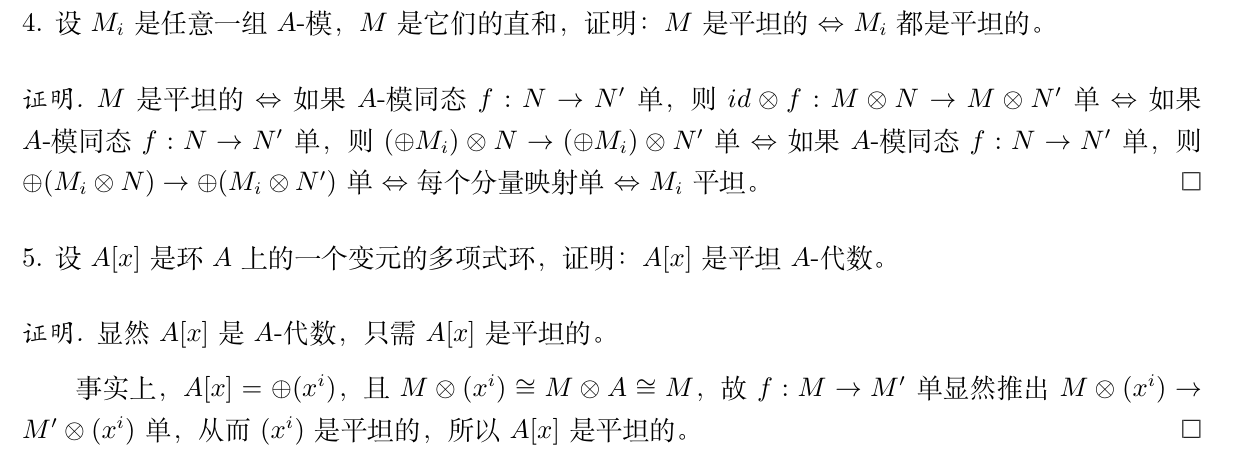
\includegraphics[width=\textwidth]{2-交换代数-2025052111.png}
% \caption{}
\label{}
\end{figure}
\end{exercise}
证明中指出 "$A[x] = \bigoplus_{i \geq 0} (x^i)$"。这里 $(x^i)$ 指的是由 $x^i$ 生成的 $A$-子模,即 $A \cdot x^i = \{ax^i \mid a \in A\}$。

作为 $A$-模,$A[x]$ 是所有形如 $a_0 + a_1x + a_2x^2 + \cdots + a_nx^n$(其中 $a_j \in A$)的多项式的集合。它可以看作是 $A$-模 $A \cdot 1$,$A \cdot x$,$A \cdot x^2$,… 的直和:
\[
A[x] = A \cdot 1 \oplus A \cdot x \oplus A \cdot x^2 \oplus \cdots = \bigoplus_{i \geq 0} A \cdot x^i.
\]
这意味着 $A[x]$ 是一个自由 $A$ -模,其基为 $\{1, x, x^2, \ldots\}$。
